\documentclass{article}

%\usepackage{corl_2023} % Use this for the initial submission.
\usepackage[final]{corl_2023} % Uncomment for the camera-ready ``final'' version.
%\usepackage[preprint]{corl_2023} % Uncomment for pre-prints (e.g., arxiv); This is like ``final'', but will remove the CORL footnote.

\usepackage{graphicx}
\usepackage{amssymb}
\usepackage{amsmath}
\usepackage{listings}
\usepackage{subcaption}
\usepackage{latexsym}
\usepackage{amsthm}
\usepackage{natbib}
\usepackage{listings}
\usepackage{hyperref} 

\title{Exercise 2 - Robot Learning Course}

% The \author macro works with any number of authors. There are two
% commands used to separate the names and addresses of multiple
% authors: \And and \AND.
%
% Using \And between authors leaves it to LaTeX to determine where to
% break the lines. Using \AND forces a line break at that point. So,
% if LaTeX puts 3 of 4 authors names on the first line, and the last
% on the second line, try using \AND instead of \And before the third
% author name.

% NOTE: authors will be visible only in the camera-ready and preprint versions (i.e., when using the option 'final' or 'preprint'). 
% 	For the initial submission the authors will be anonymized.

\author{
  Andrea Ongaro\\
	Computer Engineering\\
	Politecnico di Torino, Italy\\
	\texttt{s329706@studenti.polito.it} \\
  %% examples of more authors
  %% \And
  %% Coauthor \\
  %% Affiliation \\
  %% Address \\
  %% \texttt{email} \\
  %% \AND
  %% Coauthor \\
  %% Affiliation \\
  %% Address \\
  %% \texttt{email} \\
  %% \And
  %% Coauthor \\
  %% Affiliation \\
  %% Address \\
  %% \texttt{email} \\
  %% \And
  %% Coauthor \\
  %% Affiliation \\
  %% Address \\
  %% \texttt{email} \\
}


\begin{document}
\maketitle

%===============================================================================

\begin{abstract}
This article is the second in a series of three for the Reinforcement Learning laboratory course at Politecnico di Torino. In this installment, we explore the potential of Q-learning within the OpenAI Gym environment, focusing on the CartPole problem. Our analysis includes experiments with different epsilon values and various Q-table initialization strategies. 

\end{abstract}

% Two or three meaningful keywords should be added here
\keywords{Reinforcement Learning, Robots, AI} 

%===============================================================================

\section{Introduction}
\subsection{The system - CartPole-v0}
CartPole-v0 system from OpenAI is part of the classic control environment. The starting code it's been provided by \href{https://www.polito.it/personale?p=andrea.protopapa}{Andrea Protopapa} in the course of Reinforcement Learning. Information about this system is sourced from the official documentation \cite{Cart_pole} and its GitHub repository. Below is the definition provided by the authors for CartPole-v0\\ \\
\textit{This environment corresponds to the version of the cart-pole problem described by Barto, Sutton, and Anderson in “Neuronlike Adaptive Elements That Can Solve Difficult Learning Control Problem”. A pole is attached by an un-actuated joint to a cart, which moves along a frictionless track. The pendulum is placed upright on the cart and the goal is to balance the pole by applying forces in the left and right direction on the cart.\citep{Cart_pole}}

\begin{figure}[h]
	\centering
	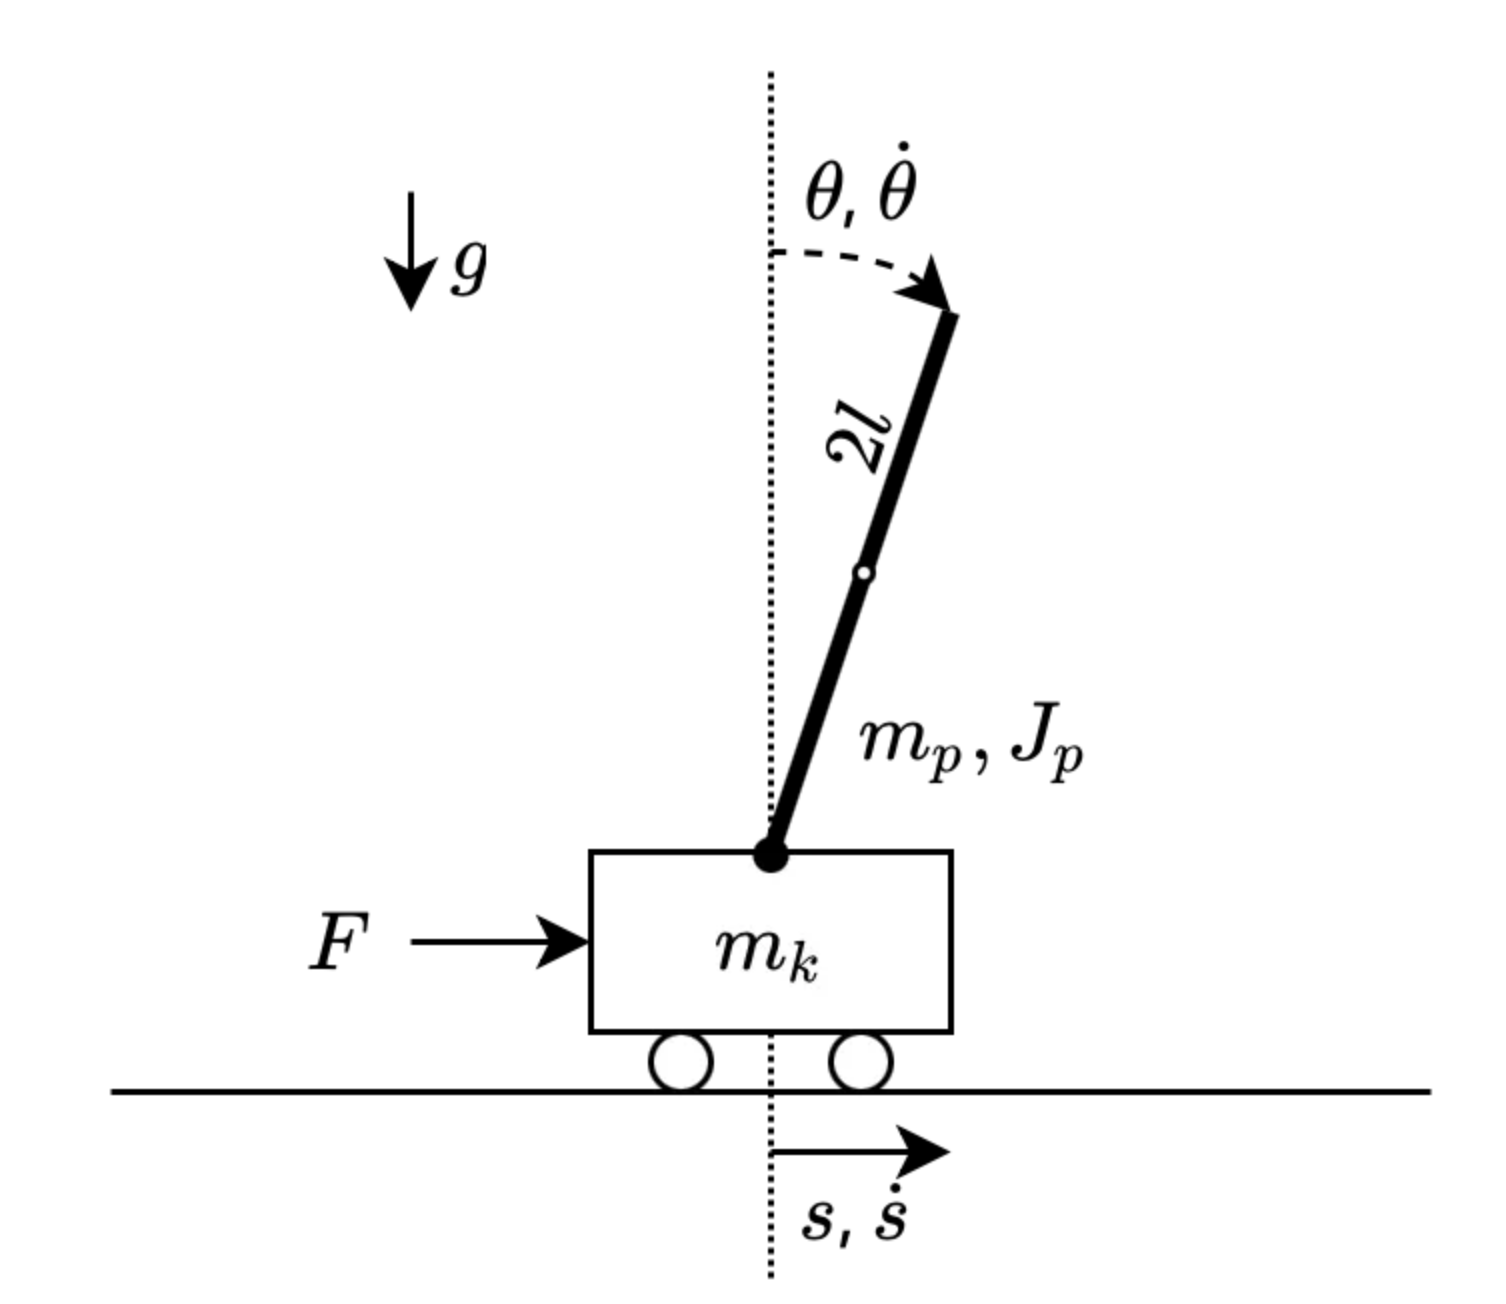
\includegraphics[width=0.5\linewidth]{../data/images/cart.png}
	\caption{Graphical explation about the whole system}
	\label{fig:plot1}
\end{figure}

\newpage

The observation is a four element vector: 
\begin{figure}[h]
	\centering
	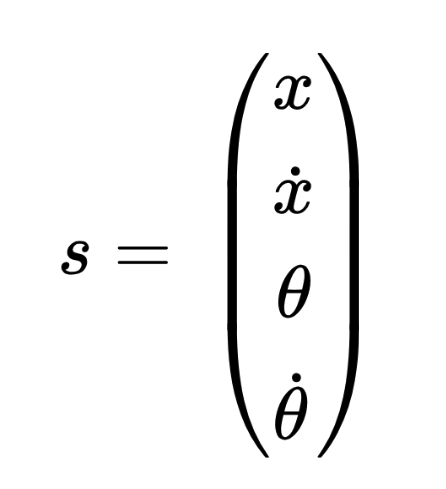
\includegraphics[width=0.2\linewidth]{../data/images/vector.png}
	\caption{Observation vector}
	\label{fig:plot1}
\end{figure}

where 
\begin{itemize}
	\item $x$: the position of the cart
	\item $\dot{x}$: the velocity, 
	\item $\theta$:  the angle of the pole
	\item $\dot{\theta}$: the angular velocity of the pole., 	
\end{itemize}

\subsection{Q-Learning}
Q-learning is a model-free algorithm. We can think of model-free algorithms as trial-and-error methods. The agent explores the environment and learns from outcomes of the actions directly, without constructing an internal model or a Markov Decision Process.
In the beginning, the agent knows the possible states and actions in an environment. Then the agent discovers the state transitions and rewards by exploration.

\begin{figure}[h]
	\centering
	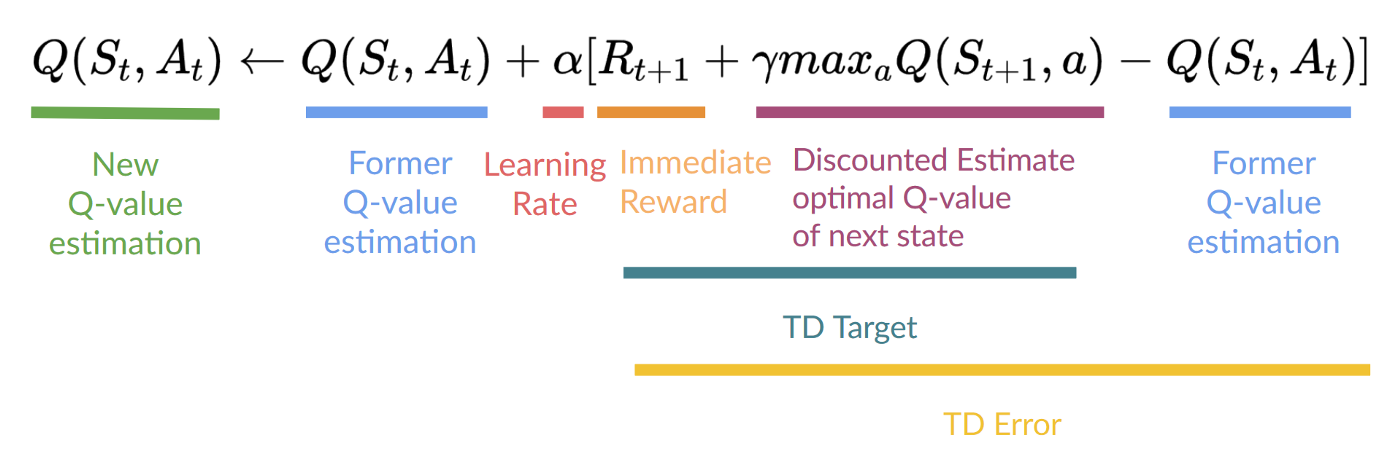
\includegraphics[width=0.5\linewidth]{../data/images/Q-learning-8.png}
	\caption{Q-value estimation}
	\label{fig:q_learning}
\end{figure}

\subsubsection{Exploration vs. Exploitation Tradeoff}
The agent tries to discover its environment. During these trials, an agent has a set of actions to select from. Some of the actions are previously selected and the agent might guess the outcome. On the other hand, some actions are never taken before.\\ \\
The concept of exploiting what the agent already knows versus exploring a random action is called the exploration-exploitation trade-off.
When the agent \textbf{explores}, it can improve its current knowledge and gain better rewards in the long run. However, when it \textbf{exploits}, it gets more reward immediately, even if it is a sub-optimal behavior.  \\ \\
As the agent can’t do both at the same time, there is a trade-off. Initially the agent doesn’t know the outcomes of possible actions. Hence, sufficient initial exploration is required. If some actions lead to better rewards than others, we want the agent to select these options. However, only exploiting what the agent already knows is a dangerous approach.

\subsubsection{$\epsilon$ greedy}
In Q-learning, we select an action based on its reward. The agent always chooses the optimal action. Hence, it generates the maximum reward possible for the given state.\\
In epsilon-greedy policy, the agent uses both exploitations to take advantage of prior knowledge and exploration to look for new options. In the figure \ref{fig:expl}, it is possible to observe how the two actions are determined.

The epsilon-greedy approach selects the action with the highest estimated reward most of the time. The aim is to have a balance between exploration and exploitation. Exploration allows us to have some room for trying new things, sometimes contradicting what we have already learned.  

With a small probability of $\epsilon$, we choose to explore, i.e., not to exploit what we have learned so far. In this case, the action is selected randomly, independent of the action-value estimates.
As we’ve discussed above, usually the optimal action, i.e., the action with the highest Q-value is selected. Otherwise, the algorithm explores a random action.

\begin{figure}[h]
	\centering
	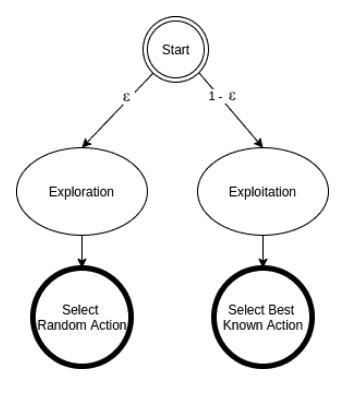
\includegraphics[width=0.5\linewidth]{../data/images/exp_e.png}
	\caption{Exploitation vs Exploration \cite{q_le}}
	\label{fig:expl}
\end{figure}

\subsubsection{GLIE - greedy in limit with infinite exploration}
GLIE (Greedy in the Limit with Infinite Exploration) ensures that each action is executed infinitely often in every state that is visited infinitely often, allowing for comprehensive exploration of the environment. Over time, the learning policy converges to a greedy approach with respect to the Q-value function, achieving optimal behavior with a probability of 1.

%Each action is executed infinitely often in every state that is visited infinitely often;
%In the limit, the learning policy is greedy with respect to the Q-value function with probability 1
% https://users.ece.cmu.edu/~yuejiec/ece18813B_notes/lecture10-online-RL-GLIE.pdf

\subsubsection{Heatmap}
To analyze the current state of the system under study, a heatmap can be utilized. The heatmap depicts values for a main variable of interest across two axis variables as a grid of colored squares. The axis variables are divided into ranges like a bar chart or histogram, and each cell’s color indicates the value of the main variable in the corresponding cell range \cite{heatmap}. \\ 

Each cell can represent different states, ranging from high-value regions, which correspond to states where the agent expects to achieve high cumulative rewards (e.g., states near the upright pole position with low velocity and angular velocity), to low-value regions, which represent states likely to lead to termination or failure (e.g., the pole falling or the cart moving out of bounds).


\section{Methodology}

\subsection{Epsilon}
They're been developed three different strategies, two of which will be compared in the following paragraph. The first strategy uses a constant epsilon value of 0.2  ($\epsilon =  0.2$) while the second employs the following formula (Equation \ref{formula:epsilon} where epsilon decreases to 0.1 after 20.000 episodes. To achieve this, we set the value of b to 2221, which ensures that at the end of the GLIE schedule, epsilon will be approximately equal to $0.09995049727735025$

\centering
\label{formula:epsilon}
$ e_k = b / (b+k) $ 

\flushleft

\subsubsection{Fixed $\epsilon$ vs GLIE epsilon schedule}
When comparing the performance of a fixed epsilon (Figure \ref{fig:costant_eps}) versus the GLIE epsilon schedule (Figure \ref{fig:glie_eps}), there is not much difference between the two. Overall, the second strategy (with the GLIE epsilon schedule) starts with a lower reward, but ultimately achieves a higher one

Looking at the testing render, it is evident that the GLIE schedule leads to more frequent successful episodes compared to the fixed epsilon strategy, with the agent managing to keep the pole stable for longer durations. However, the performance is still not perfect, as the agent frequently fails to maintain stability.

%Speaking about the performance between a fixed epsilon vs. the GLIE epsilon schedule, there is no much difference between them. Overall the second reward \ref{glie_eps} is initially lower but it finally achieve an higher one. 
%Looking at the testing render you can see an improvement compared to the fixed epsilon it happen more times than the first to arrive at the end of the episode succeding in mantaining the pole stable, but it's not perfect anyway.

\begin{figure}[h]
	\centering
	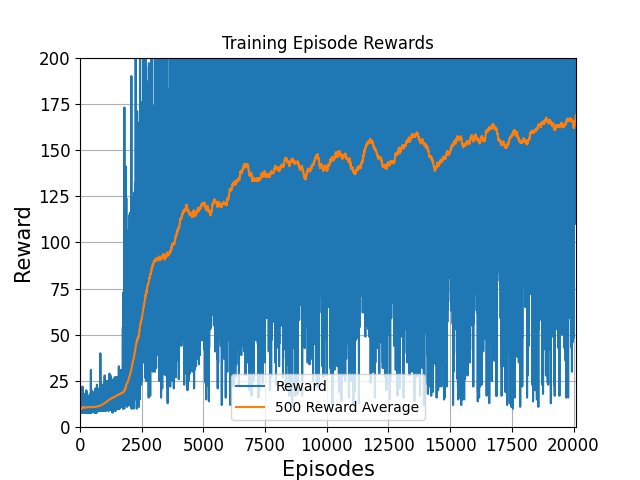
\includegraphics[width=0.5\linewidth]{../data/plot/q_learning_constant_0.2.png}
	\caption{Reward obtained - $\epsilon = 2$}
	\label{fig:costant_eps}
\end{figure}

\begin{figure}[h]
	\centering
	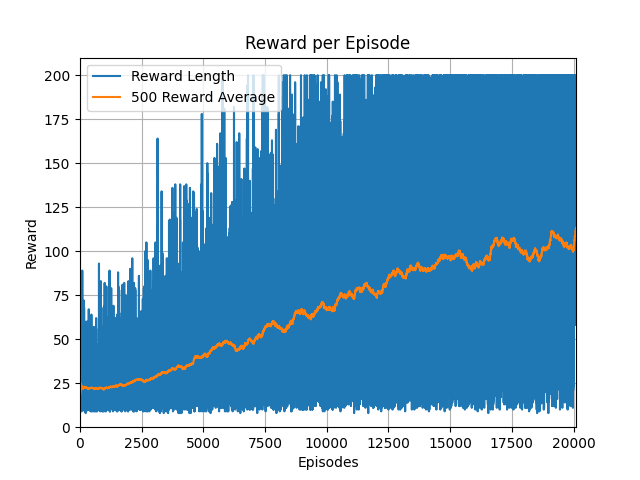
\includegraphics[width=0.5\linewidth]{../data/plot/q_learning_GLIE.png}
	\caption{Reward obtained - Formula \ref{formula:epsilon}}
	\label{fig:glie_eps}
\end{figure}

\subsection{Value function}
After computing the associated value function, the heatmap of the computed value function in terms of $ x $ and $\dot{\theta}$,(the current position of the cart and the pole angle) was generated. To plot this, the values were averaged over $\dot{x} $ and $\dot{\theta} $.

Analyzing  the full training heatmaps, one for the constant epsilon strategy (Figure  \ref{fig:heatmap_costant_full}) and the other for the GLIE schedule (Figure \ref{fig:heatmap_glie_full}), it is clear that the agent has effectively learned the optimal policy. The heatmaps are smooth and clear, with distinct high-value regions corresponding to optimal states or policies. 

\begin{figure}[h]
	\centering
	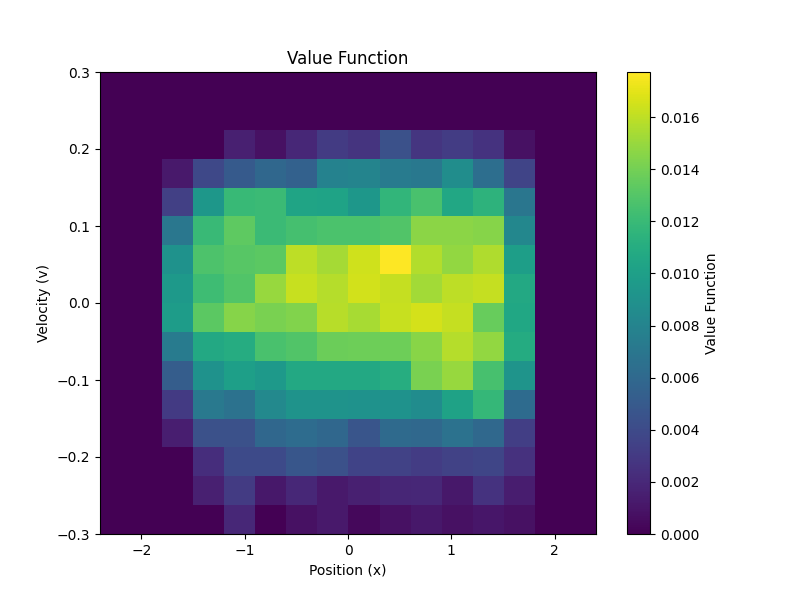
\includegraphics[width=0.5\linewidth]{../data/plot/heatmap_full_training_constant_0.2.png}
	\caption{Heatmap image for q-learning with costant epsilon}
	\label{fig:heatmap_costant_full}
\end{figure}
\begin{figure}[h]
	\centering
	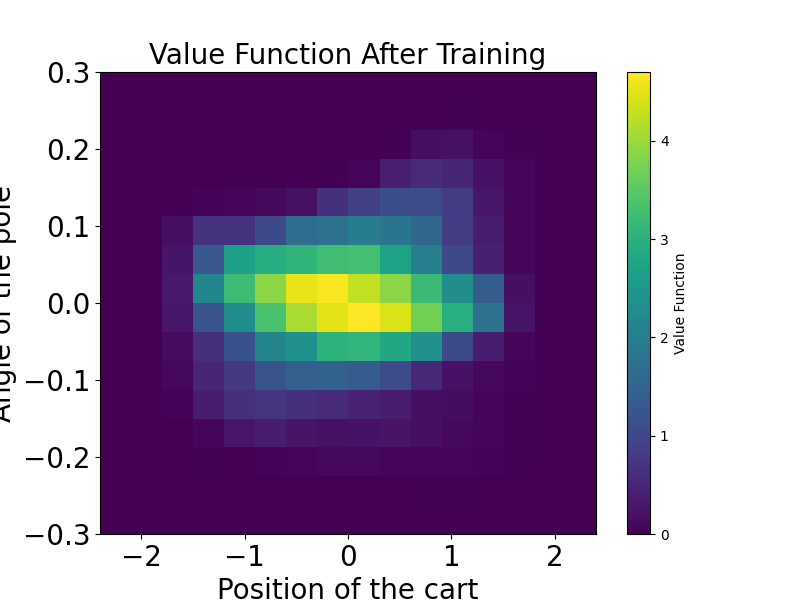
\includegraphics[width=0.5\linewidth]{../data/plot/heatmap_full_training_GLIE.png}
	\caption{Heatmap image for q-learning with glie epsilon schedule}
	\label{fig:heatmap_glie_full}
\end{figure}

Next, the focus will be on analyzing the constant epsilon case, specifically examining the Q-value heatmap at different stages of the training: before training, after a single episode, and after half of the episodes.

The general trend is consistent. These heatmaps can be found in the data/plots folder for further analysis.


\subsubsection{Before training}
Before training the heatmap is likely flat, with no clear structure. All state-action pairs have equal zero Q -values, meaning  the value function is uniform across states. The agent has no prior knowledge of the environment.

\begin{figure}[!htb]
	\begin{minipage}{0.48\textwidth}
		\centering
		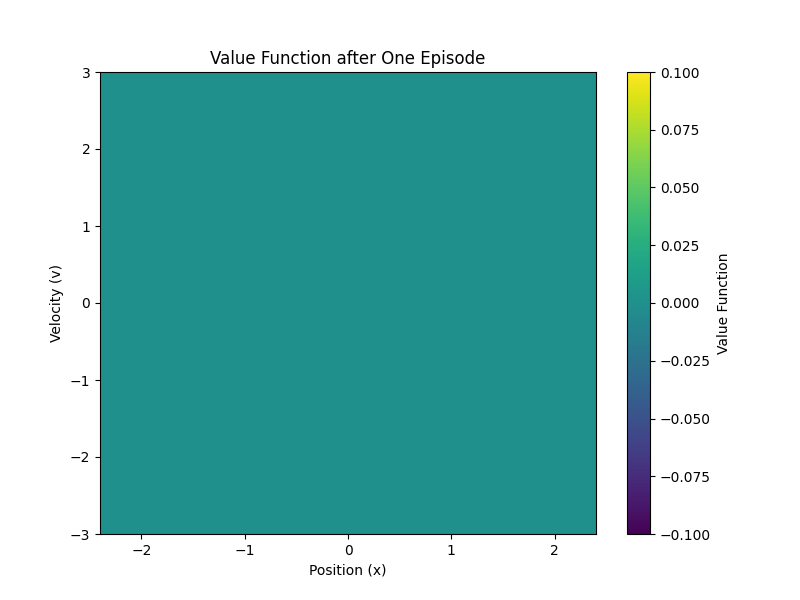
\includegraphics[width=0.5\linewidth]{../data/plot/heatmap_initial_training_constant_0.2.png}
		\caption{Heatmap in the initial state}
		\label{fig:heatmap_init}
	\end{minipage}\hfill
	\begin{minipage}{0.48\textwidth}
		\centering
		\includegraphics[width=0.5\linewidth]{../data/plot/heatmap_initial_training_glie.png}
		\caption{Heatmap in the initial state}
		\label{fig:heatmap_init}
	\end{minipage}
\end{figure}



\subsubsection{After one episode}
After one episode some regions of the heatmap may begin to show slightly higher values, particularly in states visited during the episode. The updates are sparse and localized around the trajectory the agent followed during the episode. 
Unvisited states retain their initial values, while the agent updates the Q-values for the specific states and actions it encountered, thereby improving its estimate of  V(s)  in those regions.
As a result, most of the state space remains unexplored, leading to minimal structure in the heatmap. See figure \ref{fig:heatmap_costant_init}

\begin{figure}[!htb]
	\begin{minipage}{0.48\textwidth}
	\centering
	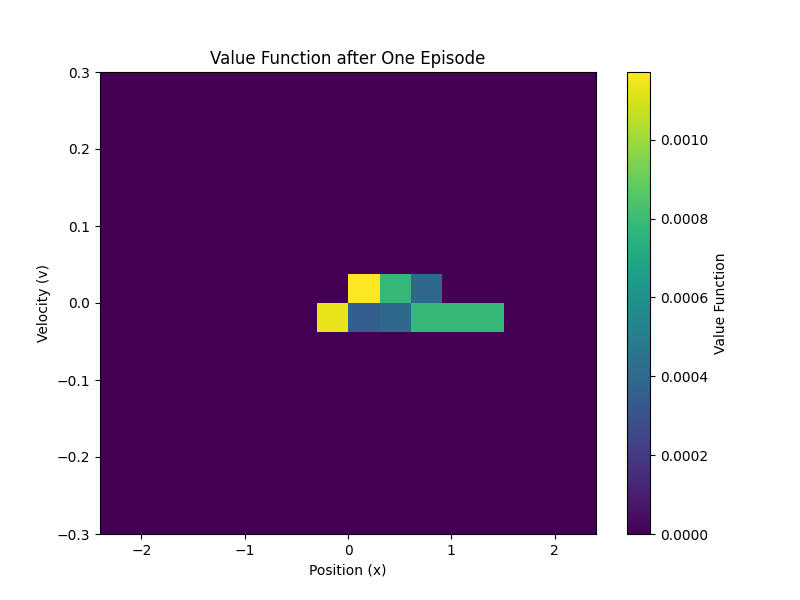
\includegraphics[width=0.5\linewidth]{../data/plot/heatmap_after_one_episode_constant_0.2.png}
	\caption{Heatmap after one single episode \\ using $\epsilon = 0.2$}
	\label{fig:heatmap_costant_init}
	\end{minipage}\hfill
	\begin{minipage}{0.48\textwidth}
	\centering
	\includegraphics[width=0.5\linewidth]{../data/plot/heatmap_after_one_episode_glie.png}
	\caption{Heatmap after one single episode \\ using Formula \ref{formula:epsilon}}
	\label{fig:heatmap_costant_init}
	\end{minipage}
\end{figure}

\subsubsection{Half-way training}
The heatmap begins to take shape, revealing a clearer distinction between “good” and “bad” states. High-value regions correspond to states that are closer to the goal or lead to higher rewards, while low-value regions represent states where the agent anticipates poor outcomes or failures. Some areas may still appear noisy or less structured, particularly in regions that have been underexplored. See figure \ref{fig:heatmap_costant_half}


\begin{figure}[!htb]
	\begin{minipage}{0.48\textwidth}
		\centering
		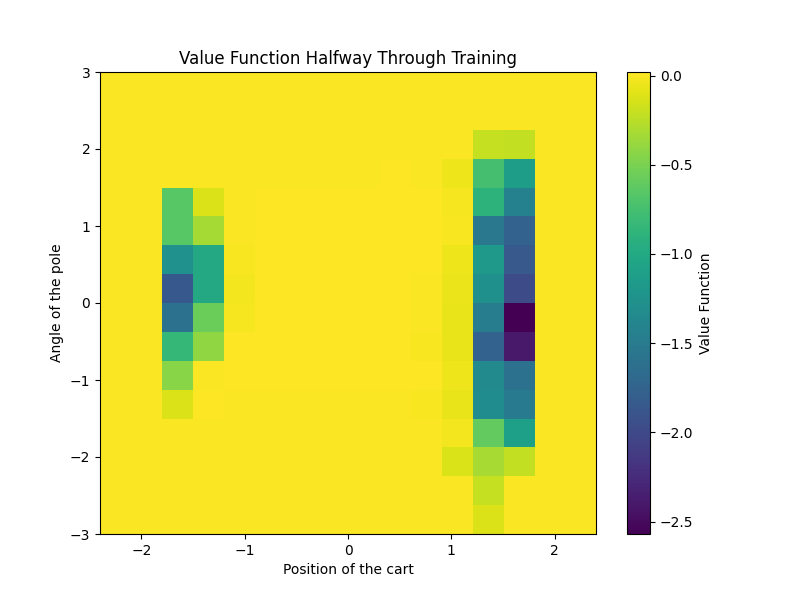
\includegraphics[width=0.5\linewidth]{../data/plot/heatmap_halfway_constant_0.2.png}
		\caption{Halfway Training Heatmap  \\ using $\epsilon = 0.2$}
		\label{fig:heatmap_costant_half}
	\end{minipage}\hfill
	\begin{minipage}{0.48\textwidth}
		\centering
		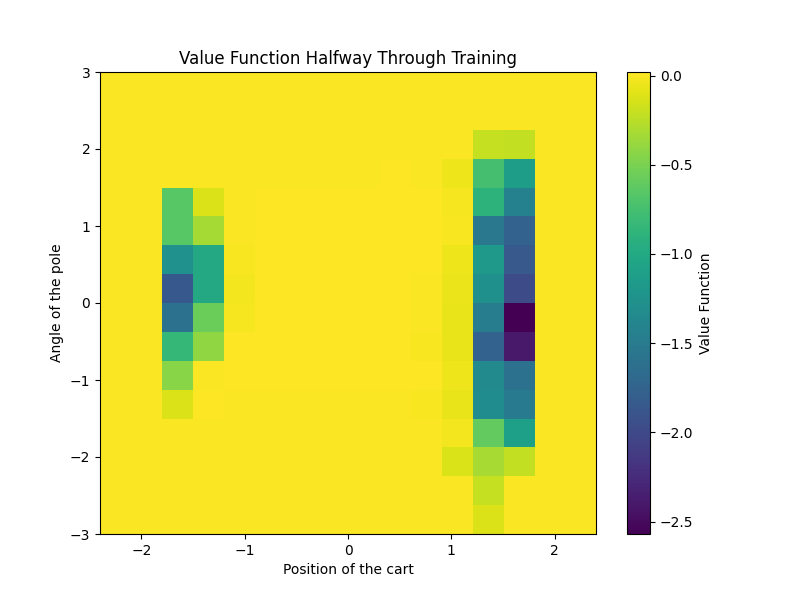
\includegraphics[width=0.5\linewidth]{../data/plot/heatmap_halfway_constant_0.2.png}
		\caption{Halfway Training Heatmap  \\ using Formula \ref{formula:epsilon}}
		\label{fig:heatmap_costant_half}
	\end{minipage}
\end{figure}

\begin{figure}[h]

\end{figure}


\subsection{Epsilon zero}
The final strategy analyzed in this article involves setting epsilon to 0. With epsilon set to 0, there is no exploration, meaning the agent relies solely on its current knowledge without attempting to discover new states or actions. Without exploration, there is no guarantee that the agent can sufficiently learn the environment to identify the optimal policy and it may stuck in \textbf{sub-optimal policy}.\\
In this subsection, the scenario of epsilon equal to zero is examined under two different cases:
\begin{itemize}
	\item keeping the initial Q-function values at zero;
	\item setting the initial Q-function values at 50 for all states and actions;
\end{itemize}

\subsubsection{Performance}
Change the initialization introduce centainlty some bias.
If Q-values are initialized to 50, the agent assumes it can achieve high rewards from all state-action pairs initially and the convergence will be slower because the updates of the Q-values will take longer to overwrite the inflated values.

The performance is poor in both cases; however, the strategy with higher initialization yields slightly better results, with longer episode durations. 

\begin{figure}[h]
	\centering
	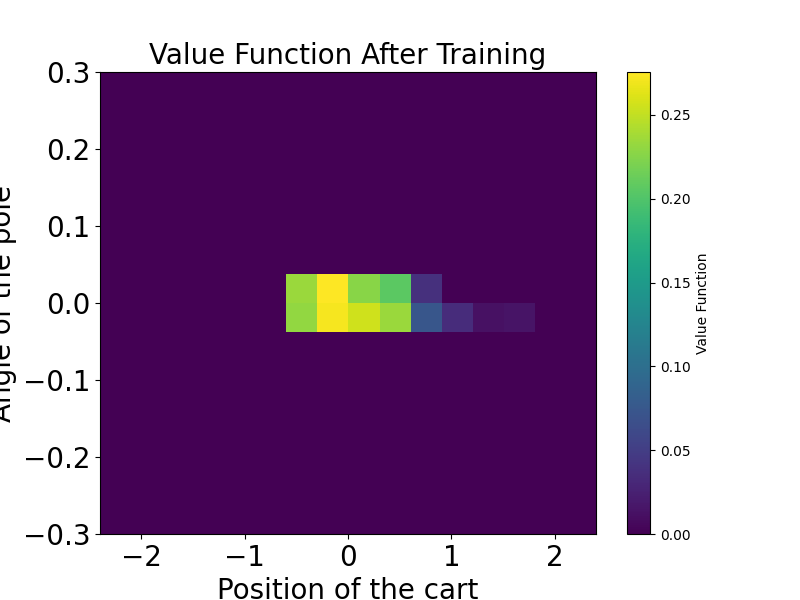
\includegraphics[width=0.5\linewidth]{../data/plot/heatmap_full_training_zero_epsilon.png}
	\caption{Full training Heatmap with epsilon zero}
	\label{fig:heatmap_zero}
\end{figure}

\begin{figure}[h]
	\centering
	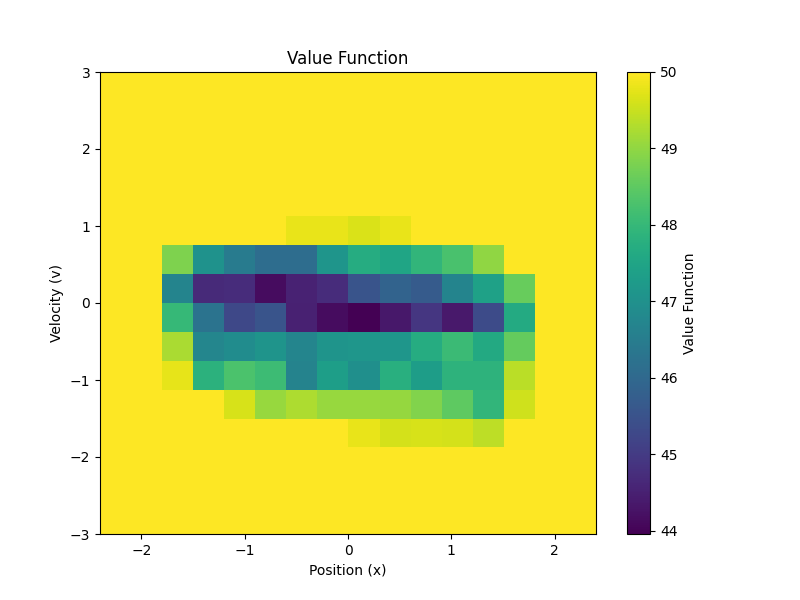
\includegraphics[width=0.5\linewidth]{../data/plot/heatmap_full_training_zero_epsilon_fifty_initial.png}
	\caption{Full training Heatmap with epsilon zero and Q values initialized at 50}
	\label{fig:heatmap_zero}
\end{figure}

\newpage

\section{Q-Learning : Different applications}

\subsection{Continuous state spaces}
Q-learning can be adapted for environments with continuous state spaces, but it requires some modifications because the algorithm inherently relies on a discrete state-action table. A common approaches for continuous State spaces
is to use a state discretization, as it's been done in this article. \\
It is important to note that discretization can result in a loss of precision and is particularly affected by the “curse of dimensionality”\cite{BELLMAN1958228} in high-dimensional spaces. \\
To overcome this problem there is an alternative that involves the use of the function approximators (e.g., neural networks, decision trees, or linear regression) to represent the Q-function Q(s, a) instead of a table. This permits to handles continuous state spaces directly without discretization and scales better to high dimensions and it's the foundation of Deep Q-Learning (DQN), where neural networks approximate $ Q(s, a) $.
 
% Divide the continuous state space into discrete bins (grids).
% Each bin represents a discrete state, and standard Q-learning operates on this discretized state space.
\subsection{Continuous action spaces}
% https://ai.stackexchange.com/questions/12255/can-q-learning-be-used-for-continuous-state-or-action-spaces
% https://www.quora.com/Why-doesn-t-Q-learning-work-with-continuous-action-spaces
The problem is can be understood easily looking the formula, the part about the TD Target (See Figure \ref{fig:q_learning})
The process for evaluating the maximum becomes less efficient and less accurate the larger the space that it needs to check.\\
If your actions are continuous, and therefore infinite, you can’t just look up which action produces the maximum q-value because there are an infinite number of actions to scan.
Unless you discretise the action space, then this becomes very unwieldy.
There are variants of Q-learning which seek to solve this problem by not only approximating Q, but also approximating the max operation. 

%===============================================================================

%===============================================================================

\section{Conclusion}

Domande non chieste:
Standard deviation è molto alta sempre mi sa.

\label{sec:conclusion}

%===============================================================================

% no \bibliographystyle is required, since the corl style is automatically used.
\bibliography{example}  % .bib

\end{document}
